\documentclass{article}
\usepackage [russian] {babel}
\usepackage {mathtext, amsmath, caption, geometry, amssymb, graphicx, wrapfig, subfig}

\captionsetup[table]{
	justification=raggedleft,
	singlelinecheck=false,
	labelsep=colon
}
\newcommand{\eds}{\mathcal{E}}

\geometry{left = 2cm, right=1cm, top=15mm, bottom=20mm}

\title{Лабораторная работа №3.4.5. \\ \textbf{Петля гистерезиса}}
\author{Данила Шеломанов, Павел Рудачихин. Б04-507}
\date{07.10.2026}
\begin {document}
\maketitle{}


\section {Аннотация} 
	
	\hspace{4mm} Целью настоящей работы является измерение параметров петель гистерезиса трёх тороидальных образцов ферромагнитных магнитомягких материалов (кремнистого железа, пермаллоя и феррита): индукция насыщения, коэрцитивное поле, остаточная индукция, дифференциальная магнитная проницаемость.
	
	В основе экспериментального метода лежит пропорциональность напряжённости магнитного поля внутри катушки и тока через неё, зависимость ЭДС от магнитной индукции, интегрирующие свойства RC-цепочки. Таким образом на экране осциллографа воспроизводится петля гистерезиса в некотором масштабе.

\section {Теоретическое введение}
	\begin{wrapfigure}{r}{0.4\textwidth}
		\centering
		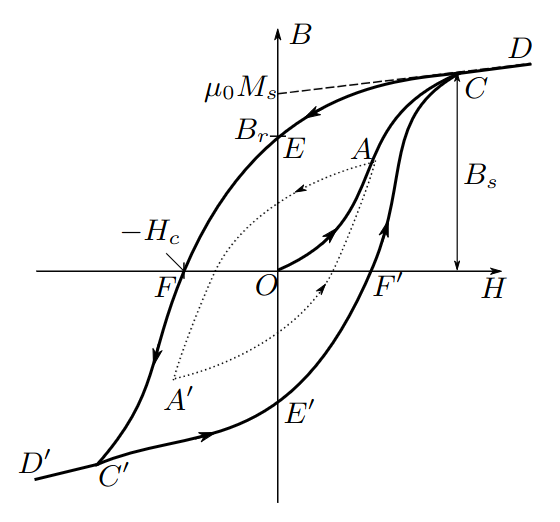
\includegraphics[width=0.38\textwidth]{loop}
		\caption{Петля гистерезиса ферромагнетика:$B_r$ -- остаточная индукция, $H_c$ -- коэрцитивное поле, OAC -- начальная кривая намагничивания.  }
		\label{fig:loop}
	\end{wrapfigure}
	\hspace{4mm} Магнитная индукция $B$ в ферромагнетике зависит не только от напряжённости поля $H$, но и от предыстории образца. Типичный график зависимости $B(H)$ для ферромагнетика представлен на рис. \ref{fig:loop}. Если к образцу прикладывать переменное внешнее магнитное поле, то его состояние в координатах HB будет меняться по замкнутой кривой -- петле гистерезиса.
	
	Концы петель гистерезиса лежат на кривой OAC. Она соответствует начальной кривой намагничивания $M(H)$ с учётом $B = \mu_0(H+M)$, где $M$ -- намагниченность, $\mu_0$ -- магнитная постоянная. Наклон кривой намагничивания характеризуется дифференциальной магнитной проницаемостью
	
	\begin{equation}
		\mu = \frac{1}{\mu_0} \frac{dB}{dH}
	\end{equation}
	
	Магнитную индукцию $B$ можно определить с помощью ЭДС, возникающей при изменении магнитного потока $\Phi$ в катушке, намотанной на образец. Если индукция однородна, то для катушки с $N$ витками и образца сечением $S$ имеем
	
	\begin{equation}
		|B| = \frac{1}{SN} \int \eds dt
	\end{equation} 

	
	Для интегрирования можно использовать RC-цепочку (см. рис. \ref{fig:RC}). Зададим следующие условия:
	
	
	
	\begin{enumerate}
		\item сопротивление источника мало по сравнению с R
		
		\item выходное сопротивление велико по сравнению с R
		
		\item сопротивление R достаточно велико, и почти всё падение напряжения приходится на него: $U_{\text{вых}} \ll U_{\text{вх}}$
	\end{enumerate}
	
	
	Пусть на вход RC-цепочки подан синусоидальный сигнал с частотой $\omega_0$, тогда отношение выходного и входного напряжений
	
	
	\begin{equation}
		\frac{U_{\text{вых}}}{U_{\text{вх}}} = \dfrac{1/(\omega_0 C)}{\sqrt{R^2 + /(\omega_0 C)^2}} = \dfrac{1}{\sqrt{(\omega_0\tau)^2 + 1}} \approx \frac{1}{\omega_0 \tau}
	\end{equation}
	\begin{wrapfigure}[]{l}{0.3\textwidth}
		\centering
		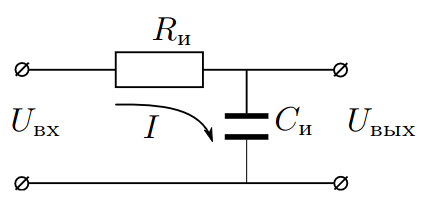
\includegraphics[width=0.28\textwidth]{RC}
		\caption{RC-цепочка}
		\label{fig:RC}
	\end{wrapfigure}
	
	Условие 3 соответствует $\tau \gg 1/\omega_0$.
	
	При таких условиях ток в цепи равен $I = (U_{\text{вх}} - U_{\text{вых}})/R \approx U_{\text{вх}}/R$, и для напряжения на выходе имеем
	
	\begin{equation}
		U_{\text{вых}} = \frac{q}{C} = \frac{1}{C} \int_{0}^{t}Idt \approx \frac{1}{\tau} \int_{0}^{t}U_{\text{вх}} dt
	\end{equation}
	
	где $\tau = RC$ -- постоянная времени RC-цепочки. Отсюда для индукции получаем
	
	\begin{equation}
		|B| = \frac{\tau}{SN} U_{\text{вых}}
	\end{equation}
	
	В работе используются тороидальные образцы ферромагнетиков. Для равномерной намагничивающей обмотки с числом витков $N_0$ и током $I$, намотанной на тор радиусом окружности R и радиусом сечения r по теореме о циркуляции имеем
	
	\begin{equation}
		H = \frac{N_0}{2\pi R} I
	\end{equation}
	
	Поле можно считать однородным при $r \ll R$.
	
	
	
	
\section{Описание установки}

	\hspace{4mm} В работе используются: автотрансформатор, понижающий трансформатор, интегрирующая RC-цепочка, амперметр, вольтметр, электронный осциллограф, делитель напряжения, образцы с двумя обмотками.
	
	
	
	\begin{figure}[h!]
		\centering
		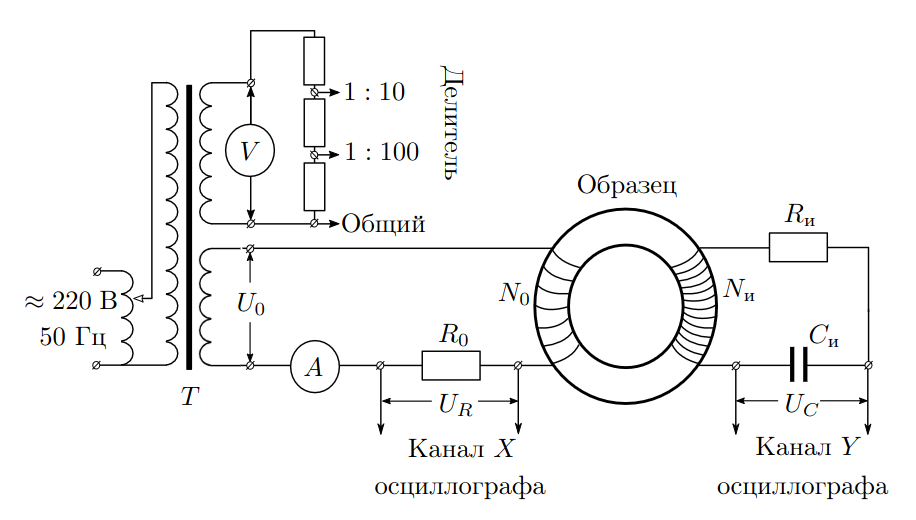
\includegraphics[width=0.7\linewidth]{setup}
		\caption{Схема установки}
		\label{fig:setup}
	\end{figure}
	
	Схема установки приведена на рис. \ref{fig:setup}. Сетевое напряжение с помощью трансформаторов Т подаётся на намагничивающую обмотку $N_0$ исследуемого образца. Последовательно этой катушке включён резистор $R_0$, напряжение $U_R$ с которого подаётся на канал X осциллографа. Амперметром А измеряется действующее значение переменного тока в намагничивающей обмотке.
	
	Напряжение с измерительной обмотки $N_{\text{и}}$ подаётся на вход RC-цепочки. Выход цепочки подключён к Y каналу осциллографа.
	
	
	
\section{Результаты и обсуждения}

	\subsection{Измерение предельных петель гистерезиса}
	
		\hspace{4mm} Путём изменения коэффициента трансформации автотрансформатора ток в намагничивающей обмотке подобран так, чтобы на осциллографе наблюдалась предельная петля гистерезиса (см.рис. \ref{fig:fullloops}): при увеличении тока площадь петли уже не меняется, увеличивается лишь длина её <<усов>>. В таком режиме измерены ширина петли по оси абсцисс $2X_c$ и высота петли по оси ординат $2Y_r$, пропорциональные коэрцитивному полю $H_c$ и остаточной индукции $B_r$ соответственно.
		
		АНАЛИЗ!
		
		
		\begin{figure}[h!]
			\centering
			\subfloat[Кремнистое железо]{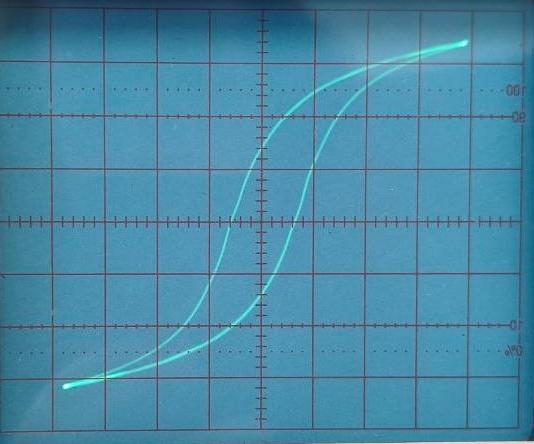
\includegraphics[width=0.3\linewidth]{Steel_full}}
			\qquad
			\subfloat[Пермаллой]{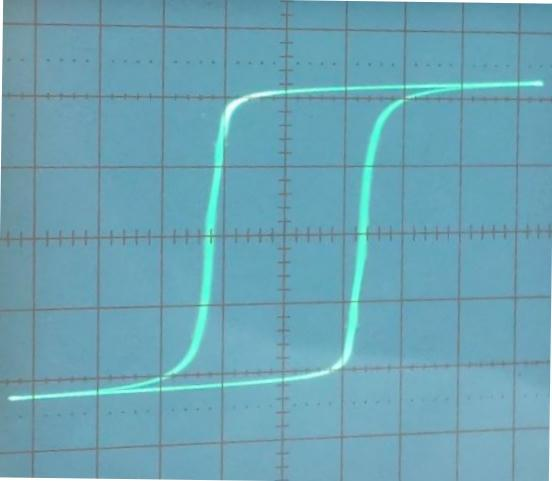
\includegraphics[width=0.3\linewidth]{Permalloy_full}}
			\qquad
			\subfloat[Феррит]{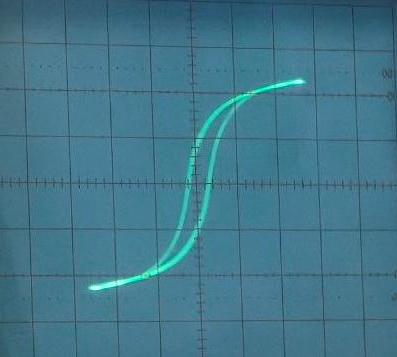
\includegraphics[width=0.3\linewidth]{Ferrit_full}}
			\caption{Предельные петли}
			\label{fig:fullloops}
		\end{figure}
		
		
		\subsection{Получение начальной кривой намагничивания}
		
		\hspace{4mm} Начиная с предельного значения тока из предыдущего подпункта, измерили ширину $2X_s$ и высоту $2Y_s$ петель, пропорциональные $H_s$ и $B_s$ соответственно, при 8--11 разных значениях тока. Некоторые виды полученных таким образом частных петель представлены на рис. \ref{fig:loops}.
		
		
		\begin{figure}[h!]
			\centering
			\subfloat[Кремнистое железо]{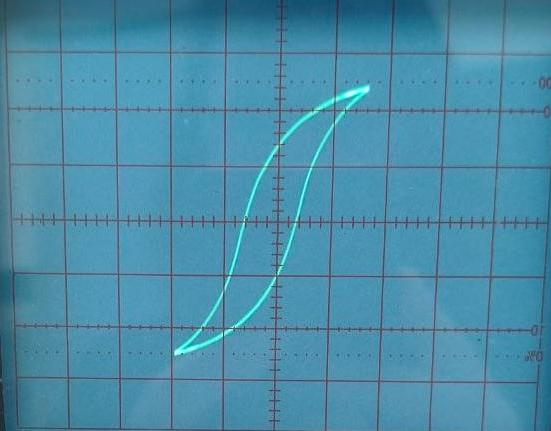
\includegraphics[width=0.3\linewidth]{Steel}}
			\qquad
			\subfloat[Феррит]{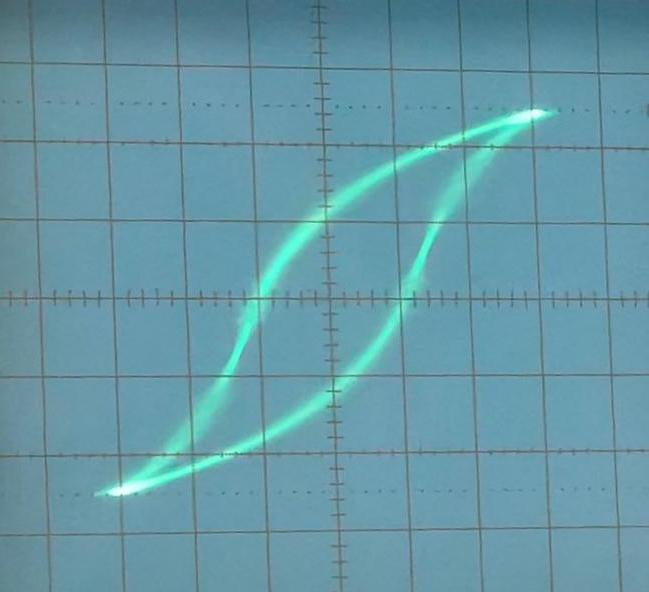
\includegraphics[width=0.3\linewidth]{Ferrit}}
			\caption{Промежуточные петли}
			\label{fig:loops}
		\end{figure}
		
		\subsection{Калибровка оси X осциллографа}
		
		\begin{figure}[h!]
			\centering
			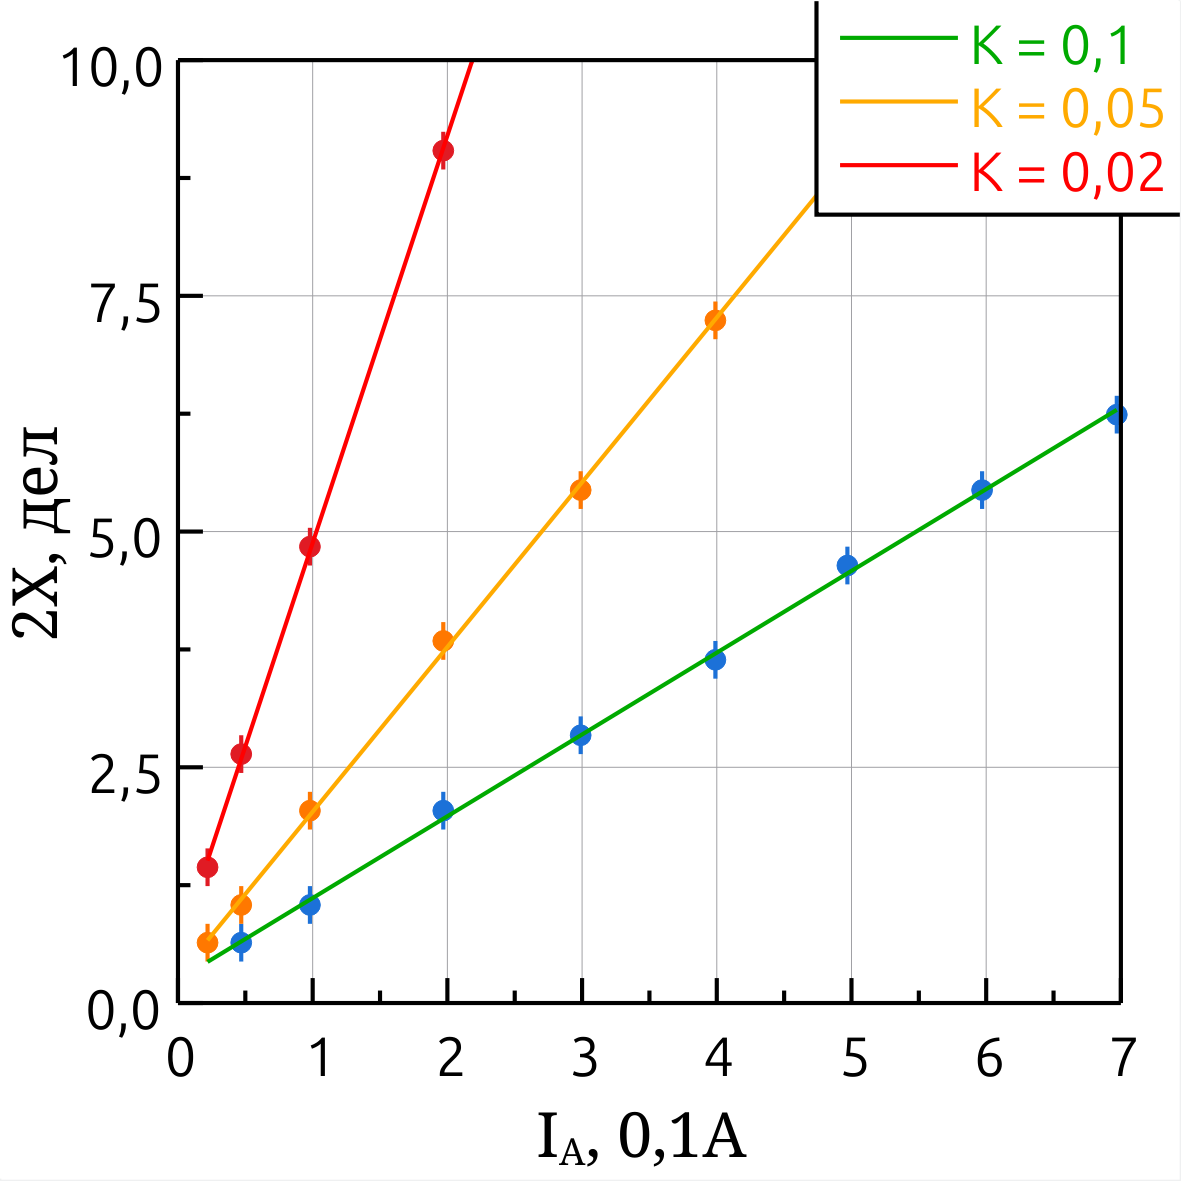
\includegraphics[width=0.4\textwidth]{calibration}
			\caption{Калибровка оси X осциллографа}
			\label{fig:calibration}
		\end{figure}
		\hspace{4mm} Для 9 значений тока $I_A$ из использованного в работе диапазона, снятых с амперметра, измерены двойные амплитуды $2X$ показаний осциллографа при разных коэффициентах усиления $K_x$ (см. рис. \ref{fig:calibration}). Из линейной аппроксимации методом наименьших квадратов получен коэффициент зависимости $2X = kI_A$ для трёх $K_x$. C учётом $I = \sqrt{2}I_A$ получен переводной коэффициент $\kappa X = I$. 
		В конечном счёте, напряжённость вычисляется так
		
		\begin{equation}
			H = \frac{N_0}{2\pi R} \kappa(K_x) X = \alpha \kappa (K_x) X
		\end{equation}
		
		где $\alpha$ определяется параметрами образца.
		
		\begin{table}
			\caption{Коэффициент $\kappa X = I$}
			\centering
			\begin{tabular}{|c|c|c|}
				\hline
				$K_x$ & $\kappa$, мА/дел & $\kappa / K_x$, мА/дел\\
				\hline
				0,1 &  325 $\pm$ 4 &  3250 $\pm$ 40  \\
				0,05 &  161,6 $\pm$ 1,8 &  3233 $\pm$ 36  \\
				0,02 &  65,5 $\pm$ 0,8  &  3275 $\pm$ 40 \\
				\hline
			\end{tabular}
		\end{table}
		
		\subsection{Калибровка оси Y осциллографа}
		
		\hspace{4mm} Канал Y осциллографа был подключён к делителю 1:100 параллельно вольтметру. Амплитуда сигнала составила (2,3 $\pm$ 0,2) деления при коэффициенте усиления $K_y =$ 0,1. Действующее напряжение на вольтметре $V = (167,4 \pm 0,3)$ мВ, значит амплитуда $U = (236,7 \pm 0,4)$ мВ. Измеренное по осциллографу $U^* = (230 \pm 20)$ мВ. При такой высокой погрешности калибровка не нужна.  
		
		
		\subsection{Постоянная времени RC-цепочки}
		
		\hspace{4mm} Постоянная времени RC-цепочки определена по отношению входного и выходного напряжения с помощью вольтметра, так как у него меньше погрешность. Она близка к определённой по номиналам R и C $\tau(RC) \approx 400$ мс.
		
		\begin{equation*}
			\tau = (432 \pm 4)\text{ мс}
		\end{equation*}
		
		\subsection{Кривая намагничивания}
		
		
		\begin{figure}[h!]
			\centering
			\subfloat[Кремнистое железо]{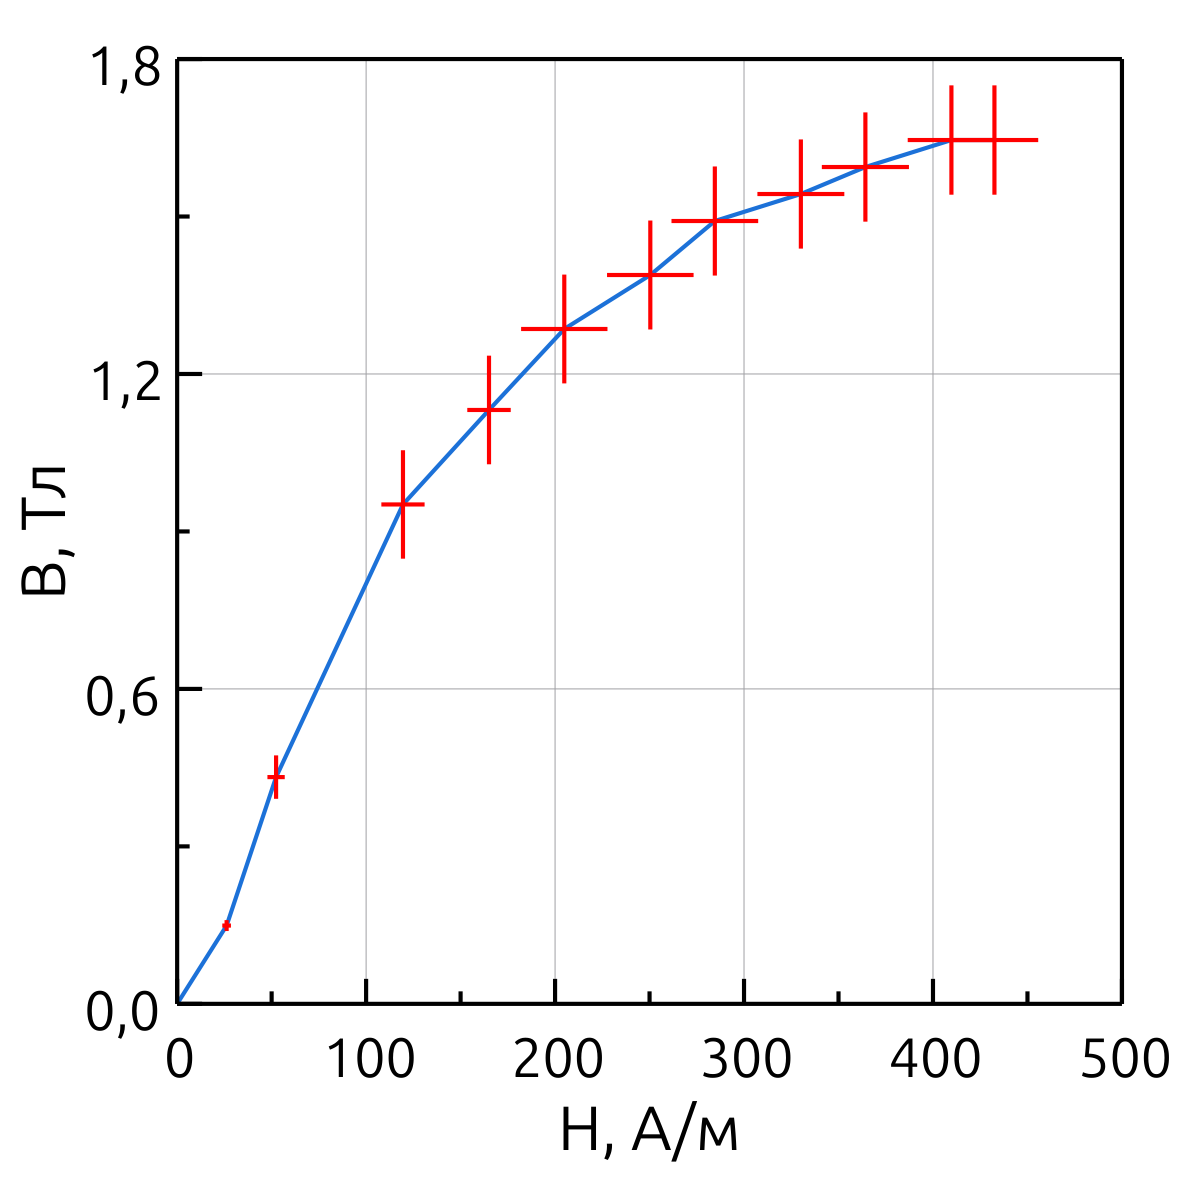
\includegraphics[width=0.3\linewidth]{FeSi}}
			\qquad
			\subfloat[Пермаллой]{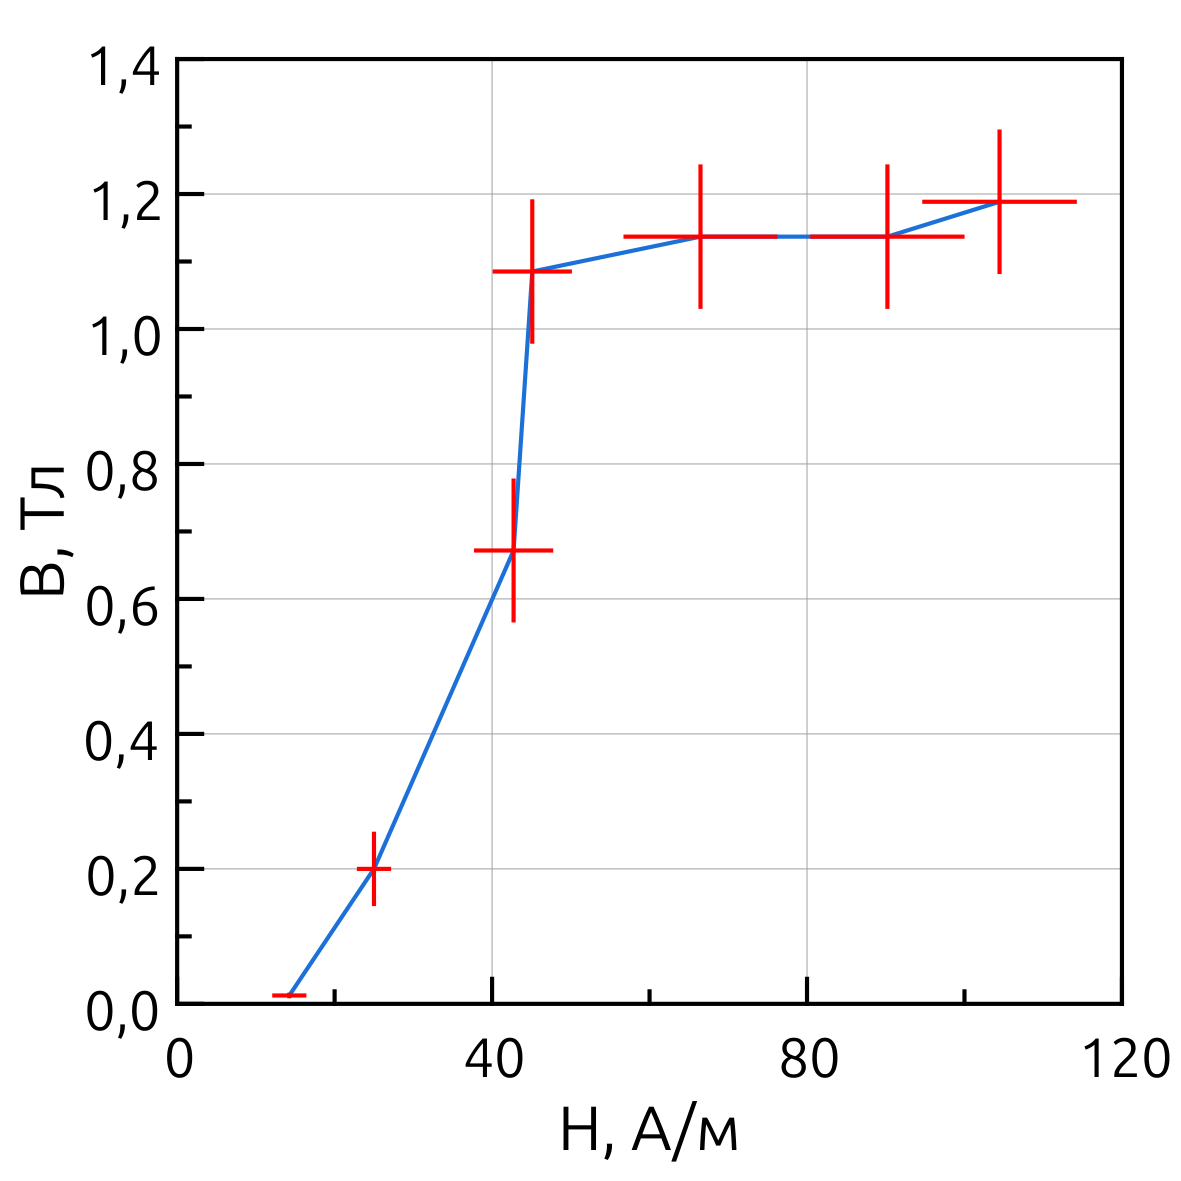
\includegraphics[width=0.3\linewidth]{Per}}
			\qquad
			\subfloat[Феррит]{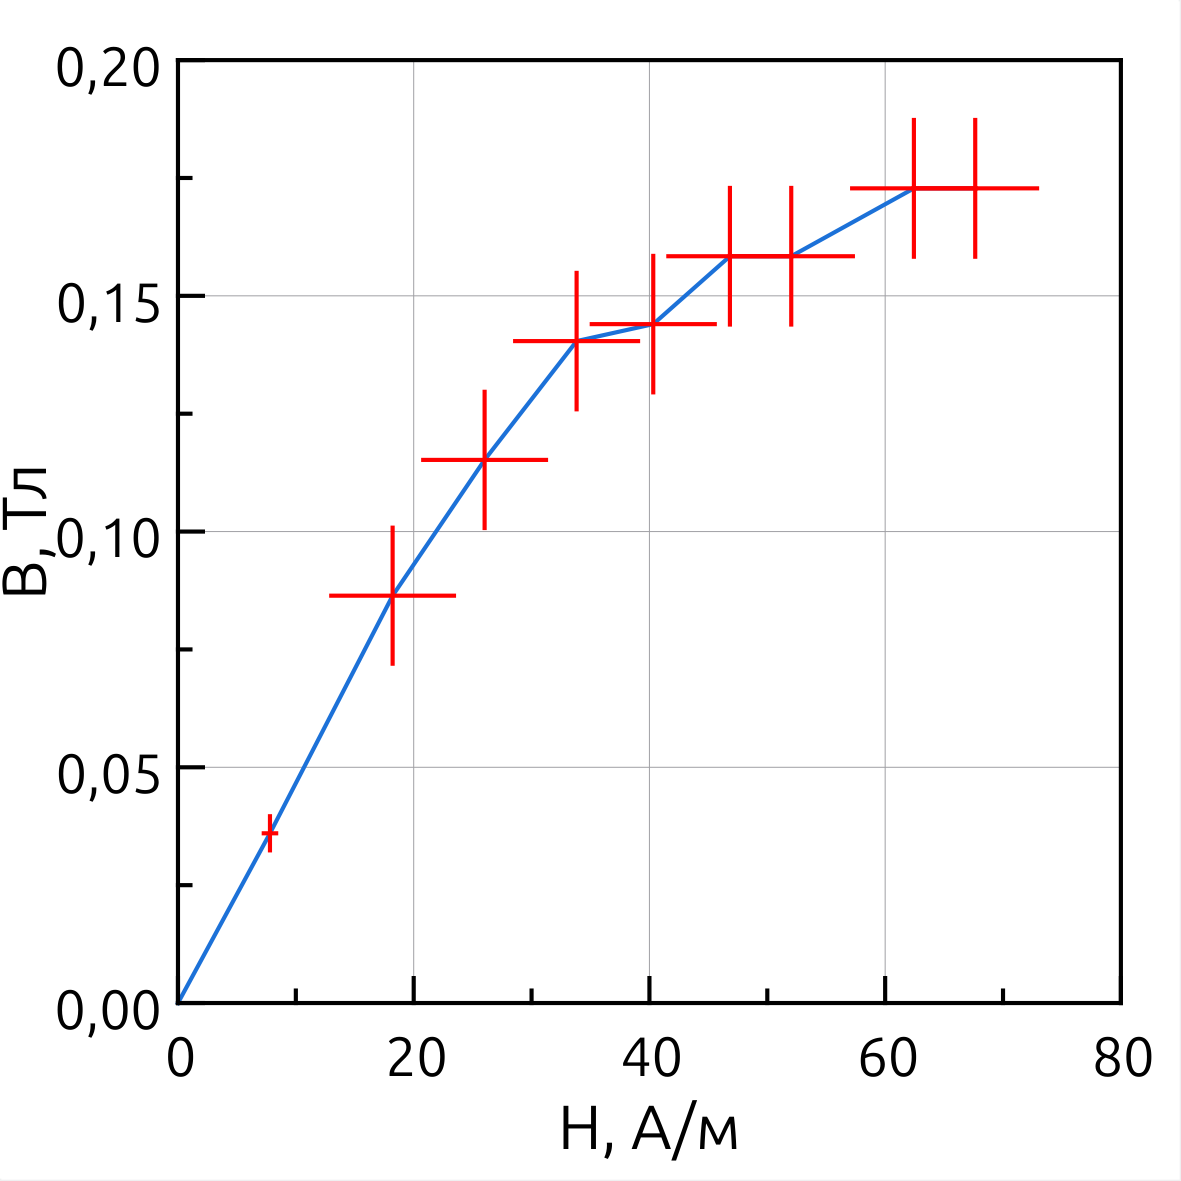
\includegraphics[width=0.3\linewidth]{Ferr}}
			\caption{Начальные кривые намагничивания B(H)}
			\label{fig:BH}
		\end{figure}
		
		\begin{figure}[h!]
			\centering
			\subfloat[Кремнистое железо]{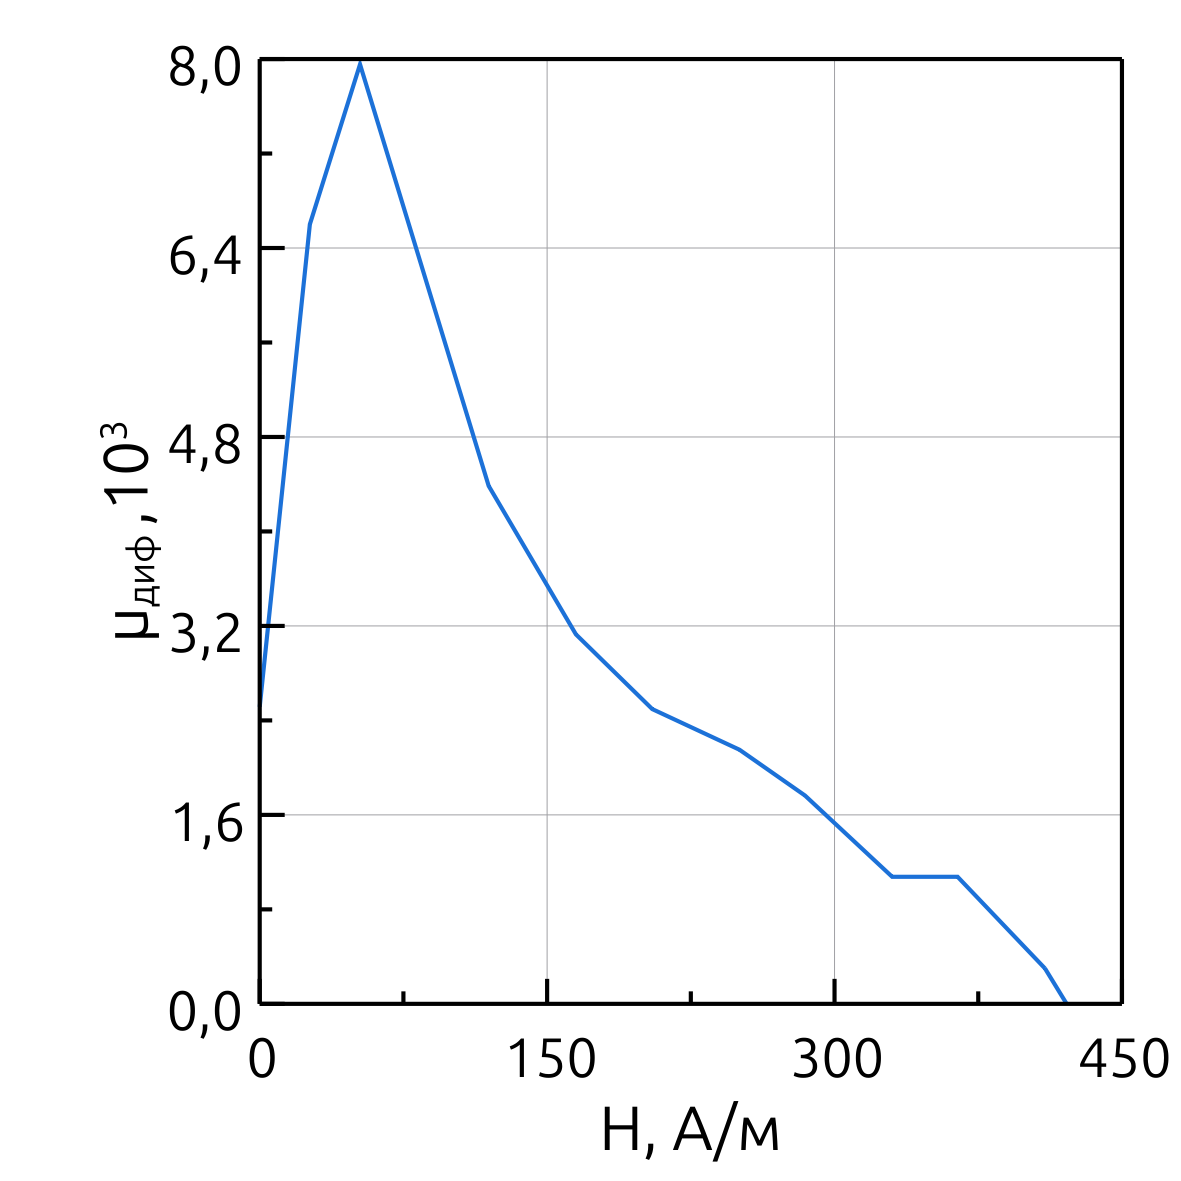
\includegraphics[width=0.3\linewidth]{FeSi_der}}
			\qquad
			\subfloat[Пермаллой]{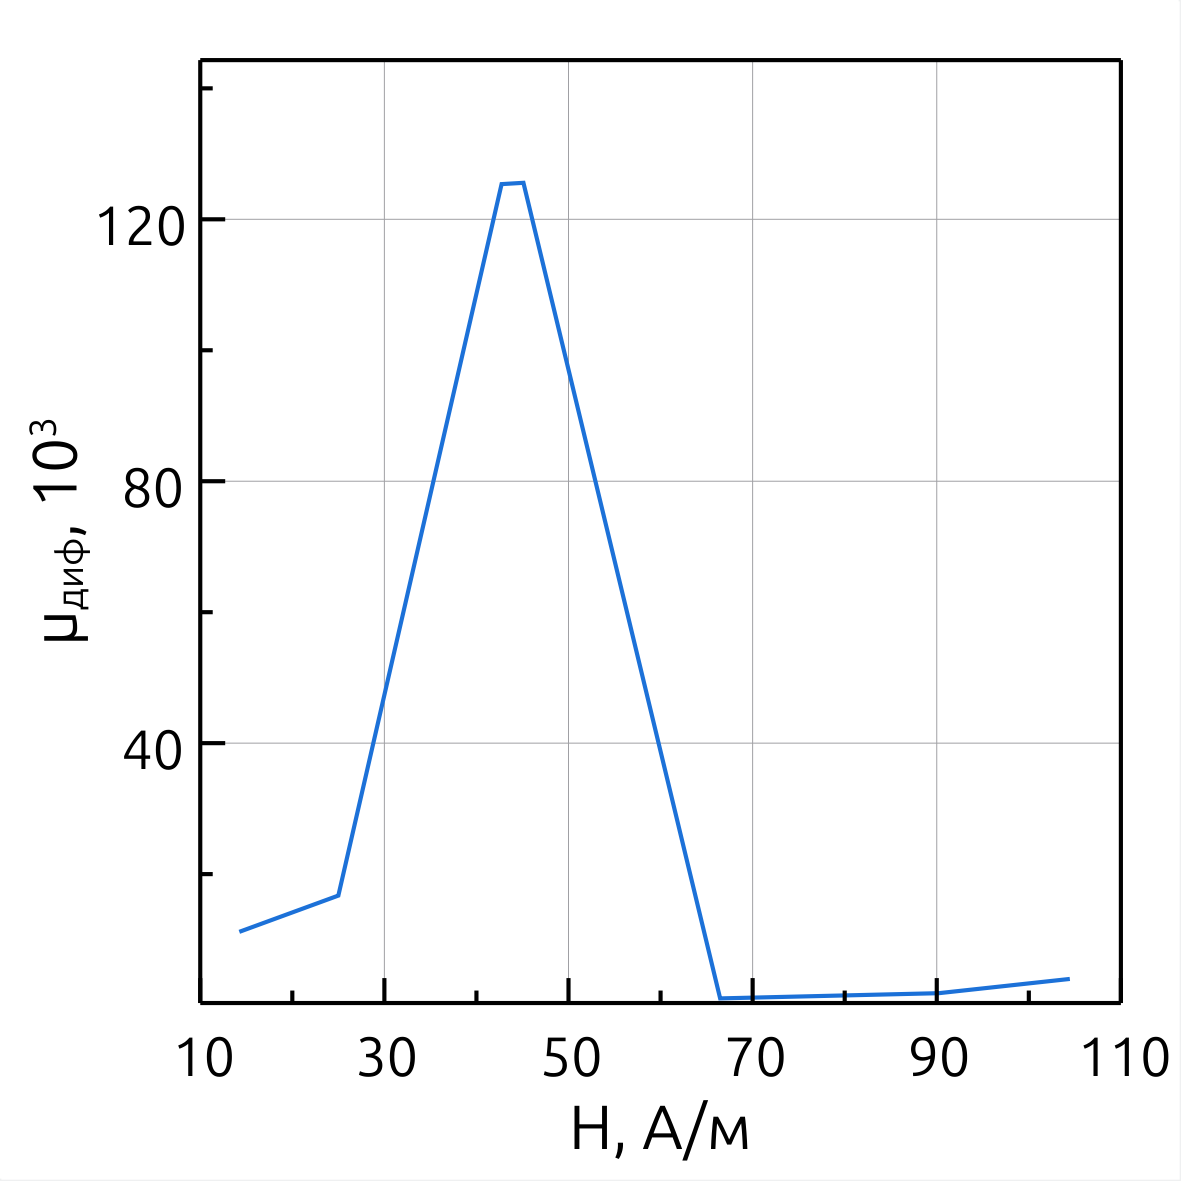
\includegraphics[width=0.3\linewidth]{Per_der}}
			\qquad
			\subfloat[Феррит]{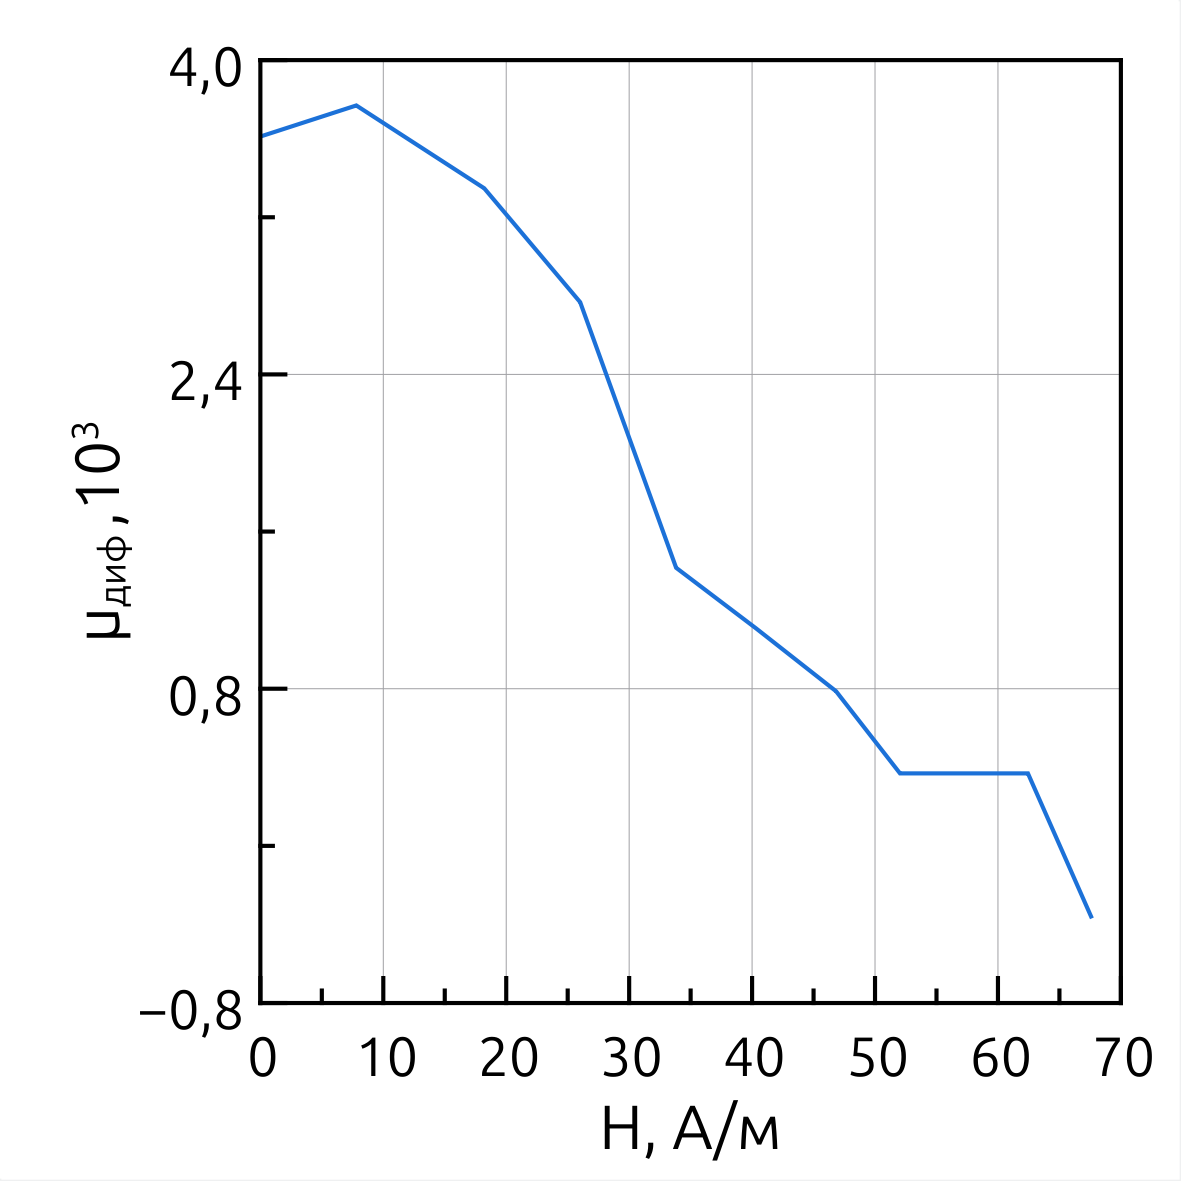
\includegraphics[width=0.3\linewidth]{Ferr_der}}
			\caption{Дифференциальная магнитная проницаемость $\mu_{\text{диф}}(H)$}
			\label{fig:muH}
		\end{figure}
		
		\hspace{4mm}По экспериментальным точкам получена кривая в координатах B(H) для трёх образцов (см. рис. \ref{fig:BH}).  Дифференцированием получена кривая $\mu_{\text{диф}}(H)$ (см. рис. \ref{fig:muH}). По ней оценены начальные и максимальные значения дифференциальной магнитной проницаемости.
		
		\begin{table}
			\caption{Параметры установки}
			\centering
			\begin{tabular}{|c|c|c|c|}
				\hline
				& Кремнистое железо & Пермаллой & Феррит \\
				\hline
				$\mu_{\text{нач}}$ & 2400 & 11 000 & 3600  \\
				\hline
				$\mu^{\text{спр}}_{\text{нач}}$ & 500 -- 9000 & 2000 -- 10 000 & 800 -- 1200 \\
				\hline
				$\mu_{\text{макс}}$&  7900 & 125 000 & 3700 \\
				\hline
				$\mu^{\text{спр}}_{\text{макс}}$ & 7000 -- 40 000& 3500 -- 100 000 & 2000 -- 3000 \\
				\hline
			\end{tabular}
			
		\end{table}
		
\section{Выводы}

	


\section{Приложение}

	\begin{table}
		\caption{Параметры установки}
		\centering
		\begin{tabular}{|r|c|}
			\hline
			Параметр & Значение \\
			\hline
			Максимальное напряжение в цепь намагничивающей катушки $U_0$ & 6,3 В  \\
			Сопротивление шунта $R_0$ & 0,3 Ом  \\
			Сопротивление резистора RC-цепочки $R_{\text{и}}$ &  20 кОм \\
			Ёмкость конденсатора RC-цепочки $C_{\text{и}}$  & 20 мкФ \\
			\hline
		\end{tabular}
	\end{table}

	\begin{table}
		\caption{Параметры образцов}
		\centering
		\begin{tabular}{|r||c|c|c|}
		\hline
		№ образца & 1 & 2 & 3 \\
		\hline
		Материал & Кремнистое железо & Пермаллой НП50 & Феррит 1000 нн\\
		\hline
		Число витков намагничивающей обмотки $N_0$ & 35 & 35 & 40 \\
		\hline
		Число витков измерительной обмотки $N_{\text{и}}$ & 350 & 220  & 400 \\
		\hline
		Площадь сечения сердечника $S$, см$^2$ & 1,2 & 3,8 & 3,0 \\
		\hline
		Длина сердечника $2\pi R$, см & 10 & 24 & 25 \\
		\hline
		Связь H(I), $\alpha = N_0 / 2\pi R$, 1/м & 350 & 146 & 160 \\
		\hline
	\end{tabular}
		
	\end{table}
	
	\begin{table}
		\caption{Измерение $\tau$}
		\centering
		\begin{tabular}{|r||c|c|}
			\hline
			 & Осциллограф & Вольтметр  \\
			\hline
			$U_{in}$, В & $11,0 \pm 1,0$ & 7,98 $\pm 0,03$ \\
			\hline
			$U_{out}$, мВ & $80 \pm 5$ & $58,8 \pm 0,3$   \\
			\hline
			$U_{out}/U_{in}$& $137 \pm 21$ & $135,7 \pm 1,2$   \\
			\hline
			$U\tau$, мс & $436 \pm 67 $ & $432 \pm 4$   \\
			\hline
		\end{tabular}
		
	\end{table}


\end {document}